\documentclass[12pt]{article}
%\usepackage{times}
\usepackage{cite}
\usepackage{indentfirst}
\usepackage{subcaption}
\usepackage{graphicx}
%this is a comment
\title{Volunteer Connector - Software Design Specification and User Interface}
\author{Daniel Domme (onid: dommed), \\
Charles Koll (onid: kollch), \\
Pedro Autran e Morais (onid: autranep), \\
Coulby Nguyen (onid: nguyenco), \\
Pavel Shonka (onid: shonkap)
}
\date{5 February 2018}

\begin{document}
\maketitle
\tableofcontents

\pagebreak
\section{User Interface Prototypes}
\subsection{Landing Page}
\begin{figure}[h!]
\includegraphics[width=\textwidth]{uiproto2}
\end{figure}
\begin{itemize}
\item
	User can login using the login button or register as a new user with the new user
	button.
\item
	While on the main page the user can filter the posts using the filter menu on the
	left side of the page. They can also click on posts to register as a volunteer.
\item
	Users can also search for certain posts using the search bar.
\end{itemize}
\pagebreak
\subsection{Logged-In Charity Page}
\begin{figure}[h!]
\includegraphics[width=\textwidth]{uiproto1}
\end{figure}
\begin{itemize}
\item
	Logged in user needs to add a photo to pop-up menu
\item
	Logged in user needs to write in a description of volunteer opportunity
\item
	Logged in user puts in application qualifications
\item
	Logged in user hits submit to add the post to database
\item
	Can also see other posts and delete or edit them
\item
	Can also browse and view applicants
\end{itemize}
\pagebreak
\subsection{Volunteers Applied Pop-up}
\begin{figure}[h!]
\includegraphics[width=\textwidth]{uiproto4}
\end{figure}
\begin{itemize}
\item
	Logged in user clicks on posting they made
\item
	Logged in user can click to see people who registered
\item
	People who registered can have accounts on the site or not
\end{itemize}
\pagebreak
\subsection{Volunteer for Event Pop-up}
\begin{figure}[h!]
\includegraphics[width=\textwidth]{uiproto3}
\end{figure}
\begin{itemize}
\item
	User can type in info and name
\item
	User hits submit to register for event
\item
	User can log in to record their submission and provide easier registration
\end{itemize}
\pagebreak
\section{Class Diagram}
\begin{figure}[h!]
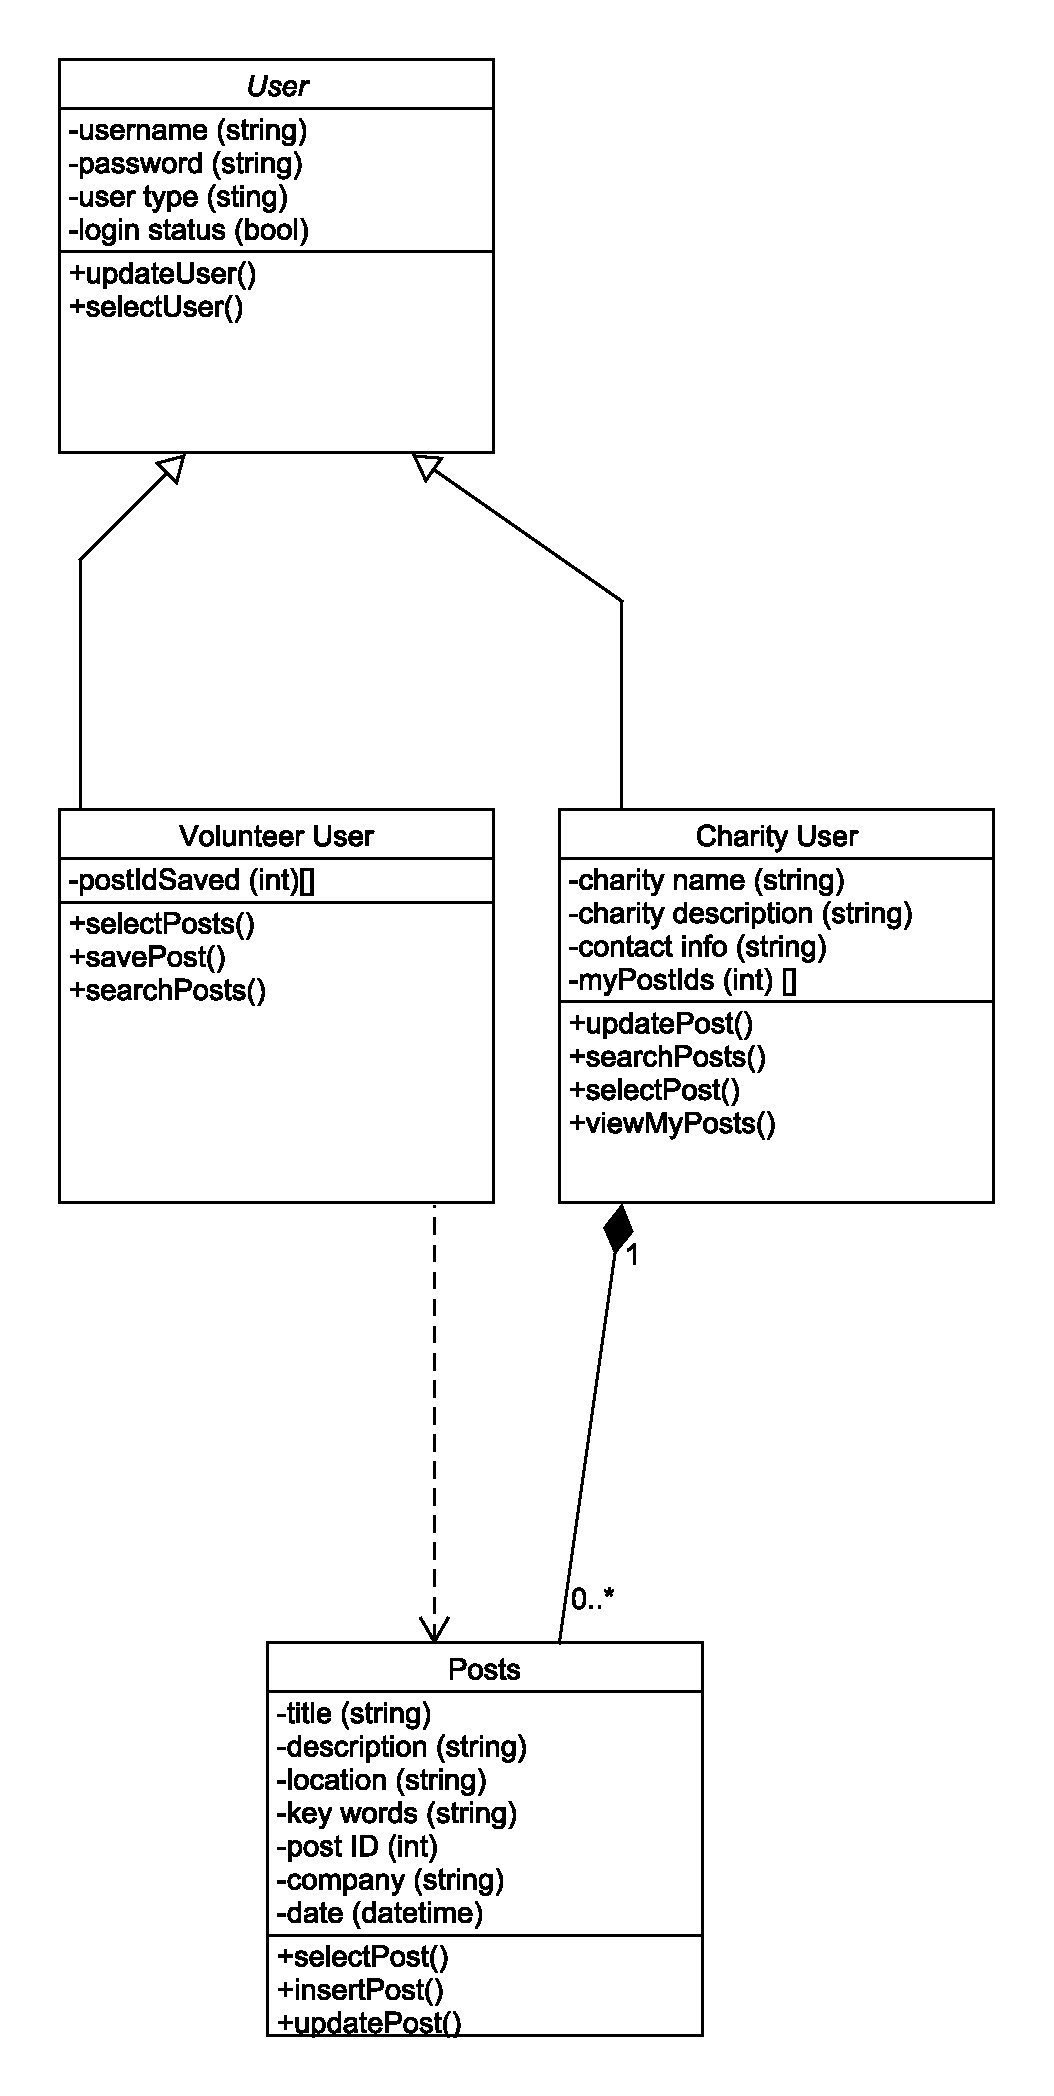
\includegraphics[width=3in]{classdiagram}
\end{figure}
\pagebreak
\section{Sequence Diagrams}
\subsection{Post Volunteer Inquiry}
\begin{figure}[h!]
\includegraphics[width=\textwidth]{usecase1}
\end{figure}
\pagebreak
\subsection{Volunteer Event Registration}
\begin{figure}[h!]
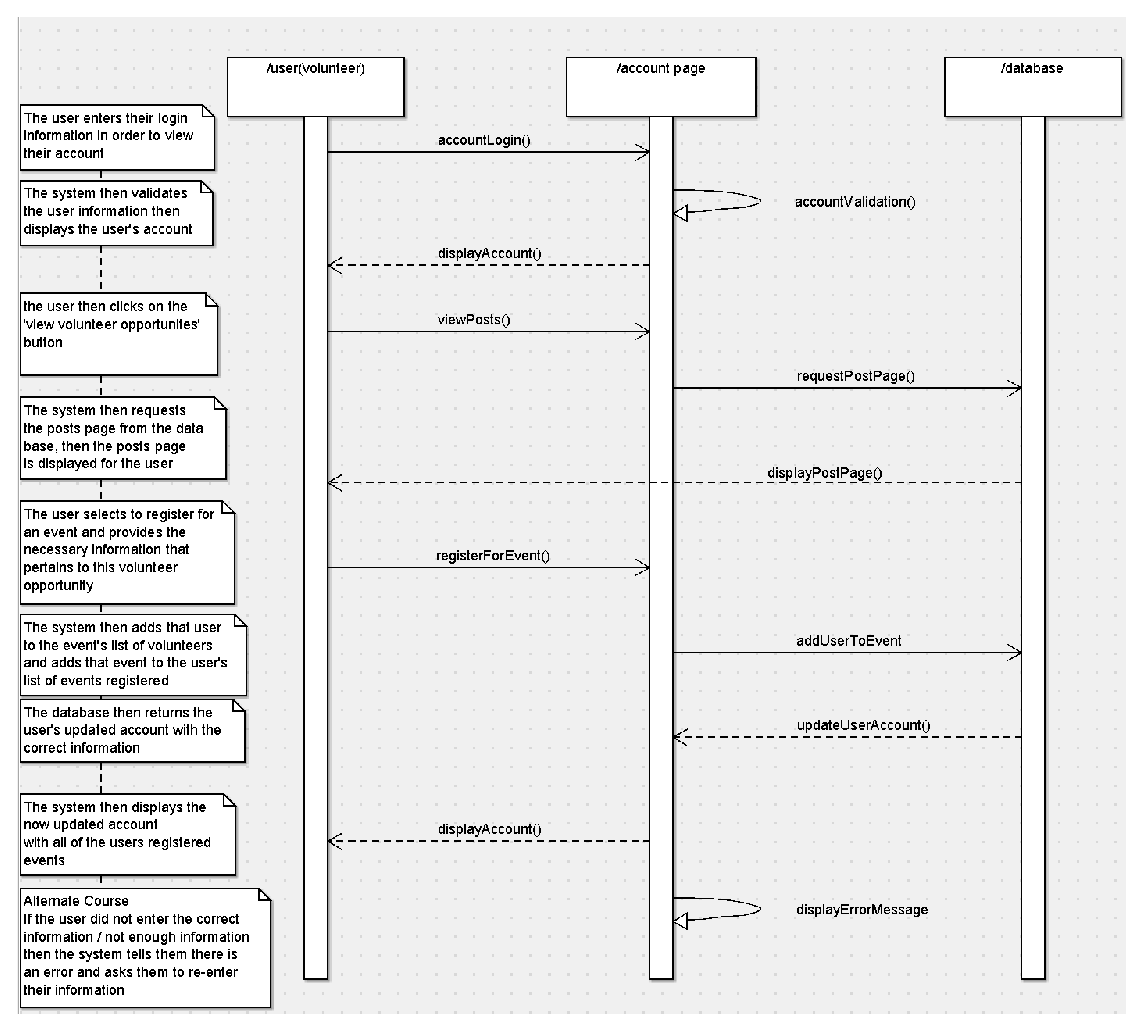
\includegraphics[width=\textwidth]{usecase2}
\end{figure}
\pagebreak
\subsection{User Search for Event}
\begin{figure}[h!]
\includegraphics[width=\textwidth]{usecase3}
\end{figure}
\pagebreak
\section{Meeting Report}
Our group met twice for this portion of the project. The first meeting was on 1 February
2018 where we outlined the final functionalities of the website. We also chose to use
node.js instead of PHP to run the site. Furthermore, the design and layout of the
website was discussed and started. On the second meeting, we discussed more design options
and put the Software Design Specification and User Interface together for turn in. For
both meetings, the customer was present and provided design input. The rest of this week,
we plan to work on fleshing out the finer details of the design of the website and the
user interface.

\quad

Division of Labor:

User Interface Prototypes: Pedro de Faria Autran e Morais, Charles Koll

Class Diagrams: Daniel Domme

Sequence Diagrams: Coulby Nguyen, Pavel Shonka

Latex Compilation: Charles Koll

\end{document}
